%!TEX program = xelatex
\documentclass[dvipsnames, svgnames,a4paper,11pt]{article}
% ----------------------------------------------------
%   中山大学物理与天文学院本科实验报告模板
%   作者:Huanyu Shi,2019级
%   知乎:https://www.zhihu.com/people/za-ran-zhu-fu-liu-xing
%   Github:https://github.com/Huanyu-Shi/SYSU-SPA-Labreport-Template
%   Last update : 2023.4.10
% ----------------------------------------------------

% ----------------------------------------------------- 
%	加边框的命令
%	参考:https://tex.stackexchange.com/questions/531559/how-to-add-the-page-border-for-first-two-pages-in-latex
\usepackage{tikz}
\usetikzlibrary{calc}
\usepackage{eso-pic}
\AddToShipoutPictureBG{%
\begin{tikzpicture}[overlay,remember picture]
\draw[line width=0.6pt] % 边框粗细
    ($ (current page.north west) + (0.6cm,-0.6cm) $)
    rectangle
    ($ (current page.south east) + (-0.6cm,0.6cm) $); % 边框位置
\end{tikzpicture}}


\usepackage{xcolor}
\definecolor{c1}{HTML}{2752C9} % 目录颜色
\definecolor{c2}{RGB}{190,20,83} % 引用颜色

\usepackage{ctex}
\usepackage[top=28mm,bottom=28mm,left=15mm,right=15mm]{geometry}
\usepackage{hyperref} 
\hypersetup{
	colorlinks,
	linktoc = section, % 超链接位置,选项有section, page, all
	linkcolor = c1, % linkcolor 目录颜色
	citecolor = c1  % citecolor 引用颜色
}
\usepackage{amsmath,enumerate,multirow,float}
\usepackage{tabularx}
\usepackage{tabu}
\usepackage{subfig}
\usepackage{fancyhdr}
\usepackage{graphicx}
\usepackage{wrapfig}  
\usepackage{physics}
\usepackage{appendix}
\usepackage{amsfonts}

%
\usepackage{tcolorbox}
\tcbuselibrary{skins,breakable}
\newtcolorbox{tbox}[2][]{
    colframe=black!70!,
    breakable,
    enhanced,
	boxrule =0.5pt,
    title = {#2},
    fonttitle = \large\kaishu\bfseries,
	drop fuzzy shadow,
    #1
}
\newtcolorbox[auto counter,number within=section]{question}[1][]{
  top=2pt,bottom=2pt,arc=1mm,
  boxrule=0.5pt,
%   frame hidden,
  breakable,
  enhanced, %跨页后不会显示下边框
  coltitle=c1!80!gray,
  colframe=c1,
  colback=c1!3!white,
  drop fuzzy shadow,
  title={思考题~\thetcbcounter:\quad},
  fonttitle=\bfseries,
  attach title to upper,
  #1
}
\newcommand{\setLhead}[1]{%
  \lhead{{\color{gray}\kaishu #1}} % 定义新的命令,设置右边页眉的内容
}
\newcommand{\setRhead}[1]{%
  \rhead{{\color{gray}\kaishu #1}} % 定义新的命令,设置右边页眉的内容
}
% ---------------------------------------------------------------------
%	利用cleveref改变引用格式,\cref是引用命令
\usepackage{cleveref}
\crefformat{figure}{#2{\textcolor{c2}{图 #1}}#3} % 图片的引用格式
\crefformat{equation}{#2{(\textcolor{c2}{#1})}#3} % 公式的引用格式
\crefformat{table}{#2{\textcolor{c2}{表 #1}}#3} % 表格的引用格式


% ---------------------------------------------------------------------
%	页眉页脚设置
\fancypagestyle{plain}{\pagestyle{fancy}}
\pagestyle{fancy}
\setLhead{中山大学物理与天文学院基础物理实验预习报告}
%\lhead{\kaishu 中山大学物理与天文学院物理实验\uppercase\expandafter{\romannumeral3}} % 左边页眉,学院 + 课程
%\rhead{{\color{gray}\kaishu Template 实验报告模板}} % 右边页眉,实验报告标题
\setRhead{实验1\hspace{1pt}冰的熔化热测量}
\cfoot{\thepage} % 页脚,中间添加页码


% ---------------------------------------------------------------------
%	对目录、章节标题的设置
\renewcommand{\contentsname}{\centerline{\huge 目录}}
\usepackage{titlesec}
\usepackage{titletoc}
% \titleformat{章节}[形状]{格式}{标题序号}{序号与标题间距}{标题前命令}[标题后命令]
\titleformat{\section}{\centering\LARGE\songti}{}{1em}{}

% ---------------------------------------------------------------------
%   listing代码环境设置
\usepackage{listings}
\lstloadlanguages{python}
\lstdefinestyle{pythonstyle}{
backgroundcolor=\color{gray!5},
language=python,
frameround=tftt,
frame=shadowbox, 
keepspaces=true,
breaklines,
columns=spaceflexible,                   
basicstyle=\ttfamily\small, % 基本文本设置,字体为teletype,大小为scriptsize
keywordstyle=[1]\color{c1}\bfseries, 
keywordstyle=[2]\color{Red!70!black},   
stringstyle=\color{Purple},       
showstringspaces=false,
commentstyle=\ttfamily\scriptsize\color{green!40!black},%注释文本设置,字体为sf,大小为smaller
tabsize=2,
morekeywords={as},
morekeywords=[2]{np, plt, sp},
numbers=left, % 代码行数
numberstyle=\it\tiny\color{gray}, % 代码行数的数字字体设置
stepnumber=1,
rulesepcolor=\color{gray!30!white}
}




% ---------------------------------------------------------------------
%	其他设置
\def\degree{${}^{\circ}$} % 角度
\graphicspath{{./images/}} % 插入图片的相对路径
\allowdisplaybreaks[4]  %允许公式跨页 % 导入模板的相关设置
\usepackage{lipsum}
\usepackage{indentfirst}
\usepackage{pdfpages}
\usepackage{multirow}
\renewcommand{\d}{\mathrm{d}}


%---------------------------------------------------------------------
%	正文
%---------------------------------------------------------------------
\setRhead{实验2-伯努利方程实验}%实验名称
\begin{document}


\begin{table}
	\renewcommand\arraystretch{1.7}
	\begin{tabularx}{\textwidth}{
		|X|X|X|X
		|X|X|X|X|}
	\hline
	\multicolumn{2}{|c|}{预习报告}&\multicolumn{2}{|c|}{实验记录}&\multicolumn{2}{|c|}{分析讨论}&\multicolumn{2}{|c|}{总成绩}\\
	\hline
	25& &30 & &25 & &80 & \\
	\hline
	\end{tabularx}
\end{table}


\begin{table}
	\renewcommand\arraystretch{1.7}
	\begin{tabularx}{\textwidth}{|X|X|X|X|}
	\hline
	专业:& 物理学类 &年级:& 2023级\\
	\hline
	姓名:& 姚昊廷  & 学号:&22322091\\
	\hline
	实验时间:& 2024.9.26& 教师签名:& \\
	\hline
	\end{tabularx}
\end{table}

\begin{center}
	\LARGE 实验2-伯努利方程实验
\end{center}

\textbf{【实验报告注意事项】}
\begin{enumerate}
	\item 实验报告由三部分组成:
	\begin{enumerate}
		\item 预习报告:(提前一周)认真研读\underline{\textbf{实验讲义}},弄清实验原理;实验所需的仪器设备、用具及其使用(强烈建议到实验室预习),完成课前预习思考题;了解实验需要测量的物理量,并根据要求提前准备实验记录表格(第一循环实验已由教师提供模板,可以打印)。预习成绩低于10分(共20分)者不能做实验。
	    \item 实验记录:认真、客观记录实验条件、实验过程中的现象以及数据。实验记录请用珠笔或者钢笔书写并签名(\textcolor{red}{\textbf{用铅笔记录的被认为无效}})。\textcolor{red}{\textbf{保持原始记录,包括写错删除部分,如因误记需要修改记录,必须按规范修改。}}(不得输入电脑打印,但可扫描手记后打印扫描件);离开前请实验教师检查记录并签名。
	    \item 分析讨论:处理实验原始数据(学习仪器使用类型的实验除外),对数据的可靠性和合理性进行分析;按规范呈现数据和结果(图、表),包括数据、图表按顺序编号及其引用;分析物理现象(含回答实验思考题,写出问题思考过程,必要时按规范引用数据);最后得出结论。
	\end{enumerate}
	\textbf{实验报告就是将预习报告、实验记录、和数据处理与分析合起来,加上本页封面。}
	\item 每次完成实验后的一周内交\textbf{实验报告}(特殊情况不能超过两周)。
	\item 除实验记录外,实验报告其他部分建议双面打印。
\end{enumerate}

{\textbf{【注意事项】}
\begin{enumerate}
	\item 实验前:要预习,明确实验目的和达成的目标;
	\item 不得随意拿取其它实验台的部件,如有缺失,请及时举手告知老师;
	\item 实验后:仔细分析处理数据,认真撰写实验报告。
\end{enumerate}}

\clearpage
\tableofcontents
\clearpage

\setcounter{section}{0}
\section{实验2-伯努利方程实验}
	
\subsection{实验目的}
\begin{enumerate}
	\item 验证伯努利能量方程,加深对机械能守恒在流体中的应用理解;通过对水力
	现象的实验分析,理解能量转换特性;
	\item 学会各种水头的测试和计量方法,掌握流速、流量、压强等水力要素的实验
	量测技能;
	\item 观察并理解毕托管测速方法的原理。
\end{enumerate}

\subsection{仪器用具}
\begin{table}[htbp]
	\centering
	\renewcommand\arraystretch{1.6}
	% \setlength{\tabcolsep}{10mm}
	\begin{tabular}{p{0.05\textwidth}|p{0.20\textwidth}|p{0.05\textwidth}|p{0.5\textwidth}}
	\hline
	编号& 仪器用具名称 & 数量 &  主要参数(型号,测量范围,测量精度等) \\
	\hline
	1&主管道实验平台 &1 &主管道、水泵、流量计、流量调节阀门\\
	\hline
	2&测压管立板  &1&测试立管$\times$13、细软管及止水夹$\times$13;注水容器、注水软管、注水调节阀门;排水管、排水止水夹 \\
	\hline
	3&水箱 & 1 &备用 \\
	\hline
	4&DC12V 电源适配器&1 & 流量计电源\\
	\hline
	5&DC 0$\sim $24V 电源适配器&1&水泵电源\\
	\hline
	6&蓝色墨水&1&非碳素不堵笔\\
	\hline
	7&温度计&1&自备,测量环境温度\\
	\hline
	8&纯净水&足量&自备\\
	\hline
\end{tabular}
\end{table}

\subsection{原理概述}
水流质点在流动的过程中具有位置高度、压力2和速度,也就是说水流质点
在流动的过程中具有位能、压能和动能3,这三种能量可用水柱高度表示。对于不
可压缩理想液体(不存在粘滞性、液体的内摩擦力为零,故所做的功也为零)来
说,水流质点从第一断面流向第二断面时这三种能量的变化关系可用伯努利方程
表示,即:
$$\frac{1}{2}\rho v_1^2+\rho gz_1+p_1=\frac{1}{2}\rho v_2^2+\rho gz_2+p_2$$
其中$\rho gz$为水流质点的位能(重力压头),$p$为压力能(静压),$frac{1}{2}\rho v^2$
为水流质点的动能(动压),下标 1、2 分别表示断面 1、2。

可进一步转换为以高度表示的伯努利方程:
$$\frac{1}{2\rho g}\rho v_1^2+z_1+\frac{p_1}{\rho g}=\frac{1}{2\rho g}\rho v_2^2+z_2+\frac{p_2}{\rho g}$$
对于实际流体,还应该考虑应黏性耗散引起的能量损失(沿程阻力损失),
则实际流体的伯努利方程为:
$$\frac{1}{2}\rho v_1^2+\rho gz_1+p_1=\frac{1}{2}\rho v_2^2+\rho gz_2+p_2+W_{1-2}$$
其中,$W_{1-2}$为水流质点从第一断面流向第二断面过程中的能量损失。

相应地,转化为以水头损失表示的伯努利方程为:
$$\frac{1}{2\rho g}\rho v_1^2+z_1+\frac{p_1}{\rho g}=\frac{1}{2\rho g}\rho v_2^2+z_2+\frac{p_2}{\rho g}+h_{1-2}$$
$h_{1-2}$为水流质点从第一断面流向第二断面过程中的水头损失。
因水流质点从一点流向另一点的过程中要消耗能量,降低水头,因此实际流
体的水头线应是一条倾斜的曲线。
选测压点(1)-(12),从相应各测压管的水面读数测得$z+\frac{p}{\rho g}$值,并计算各
测点速度水头$\frac{ v^2}{2g}$,并将各断面处的$z+\frac{p}{\rho g}$和$\frac{ v^2}{2g}$相加,测出通过管路的流量和断面
处的管径,即可计算出断面平均流速$v$及$\frac{v^2}{2g}$,从而即可得到各断面测压管水头和
总水头。
流体的沿程阻力损失可由达西公式计算,即:
$$h=\lambda\frac{L}{D}\frac{v^2}{2g}$$
公式中:$L$为管长,$D$为管径,$v$为管内平均速度,$\frac{v^2}{2g}$为速度水头。$\lambda$为沿程
摩阻系数(达西摩擦因子),$\lambda$并不是一个确定的常数,一般由实验确定。一般
情况下,$\lambda$与雷诺数$\text{R}_\text{e}$和管壁相对粗糙度有关。对于圆管内的层流流动,$\lambda=\frac{64}{\text{R}_\text{e}}$;
对于光滑圆管内的湍流流动,可用布拉休斯光滑管公式进行描述,即$\lambda=\frac{0.3164}{\text{R}_\text{e}^{0.25}}$。

毕托管利用伯努利方程原理可测出流体速度。毕托管有两根细管。一管孔口
正对液流方向,90 度转弯后液体的动能转化为势能,液体在管内上升的高度即
为该处的总水头$\frac{1}{2\rho g}\rho v^2+z+\frac{p}{\rho g}$
;而另一根管开口方向与液流方向垂直,只测量到液
体的压力,液体在管内上升的高度为该处的测压管水头(相对应于势能的那部分
水头)$z+\frac{p}{\rho g}$,两管液面的高差就是该处的流速水头$\frac{1}{2\rho g}\rho v^2$,量出两管液面的高差
$\Delta h$则$\frac{v^2}{2g}=\Delta h$,即$v=\sqrt{2g\Delta h}$,从而间接地测出该处的液体流速$v$。
\subsection{实验前思考题}
\begin{question}
	什么叫层流湍流?
	\tcblower
	层流是流体的一种流动状态。
	当流速很小时,流体分层流动,互不混合或很少部分混合称为层流,
	或称为片流;逐渐增加流速,流体的流线开始出现波浪状的摆动,
	摆动的频率及振幅随流速的增加而增加,此种流况称为过渡流;
	当流速增加到很大时,流线不再清楚可辨,流场中有许多小漩涡,
	称为湍流,又称为乱流、扰流或紊流。这种变化可以用雷诺数来量化,公式为
	$$\text{R}_\text{e}=\frac{\rho uD_H}{\mu}=\frac{uD_H}{\nu}=\frac{QD_H}{\nu A}$$
	其中,$D_H$是管道的水力直径,$Q$是体积流率;$A$是管道的横截面积,$u$流体的平均速度;$\mu$
	是流体的动力粘度;$\nu$是流体的运动粘度,$\nu=\frac{\mu}{\rho}$;$\rho$是流体的密度。

	雷诺数较小时,黏滞力对流场的影响大于惯性力,流场中流速的扰动会因黏滞力而衰减,流体流动稳定,为层流;反之,若雷诺数较大时,惯性力对流场的影响大于黏滞力,流体流动较不稳定,流速的微小变化容易发展、增强,形成紊乱、不规则的湍流流场。
	流态转变时的雷诺数值称为临界雷诺数。一般管道雷诺数$\text{R}_\text{e}<2100$为层流状态,$\text{R}_\text{e}>4000$为湍流状态,$2100<\text{R}_\text{e}<4000$时为过渡状态
\end{question}

\begin{question}
	管两侧的水头(4号与5号测压管、7号与8号测压管)是否相等?为什么?
	\tcblower
	不相等,流速大时会产生湍流,进而导致有垂直于管轴线的速度。
\end{question}

\begin{question}
	文丘里管两端的水头(1号与3号测压管)是否相等?为什么?
	\tcblower
	不相等,这两个测量点由于文丘里管的摩擦导致水头有所损失。
\end{question}

\begin{question}
	测量动压时,位置6与9哪个更合适?
	\tcblower
	9更合适,到后期速度更加稳定趋向于平均速度。
\end{question}

\begin{question}
	摩擦压降与什么因素有关?
	\tcblower
	\begin{enumerate}
		\item 液体雷诺数;
		\item 管壁摩擦系数。
	\end{enumerate}
\end{question}


\clearpage
\setLhead{中山大学物理与天文学院基础物理实验记录}
\begin{table}
	\renewcommand\arraystretch{1.7}
	\centering
	\begin{tabularx}{\textwidth}{|X|X|X|X|}
	\hline
	专业:& 物理学类 &年级:& 2023级 \\
	\hline
	姓名:& 姚昊廷 &学号:&22322091  \\
	\hline
	室温:&21$^\circ$C&实验地点:&A517\ B6\\
	\hline
	学生签名:& & 评分: &\\
	\hline
	实验时间:& 2024.9.26& 教师签名:&\\
	\hline
	\end{tabularx}
\end{table}

\section{实验2-伯努利方程实验}
\subsection{实验内容、步骤、结果}
\begin{table}[!h]
	\renewcommand\arraystretch{1.7}
	\centering
	\begin{tabularx}{\textwidth}{|c|c|X|X|X|X|X|X|X|X|X|}
	\hline
	\multicolumn{2}{|c|}{流量计流量/($\text{L}\cdot\text{min}^{-1}$)} & 0.5 & 0.65 & 0.8 & 0.95 & 1.1 & 1.25 & 1.4 & 1.55 \\ \hline
	\multirow{13}{*}{测压管水柱高度/mm} & 1($\phi 8\text{mm}$)& 545.5 & 557.9 & 572 & 585.5 & 597.9 & 616.9 & 637.2 & 657.8 \\ \cline{2-10}
	& 2($\phi 4\text{mm}$) & 511.8 & 504 & 491.1 & 476.5 & 457.5 & 438.5 & 414.5 & 389.2 \\ \cline{2-10}
	& 3($\phi 8\text{mm}$) & 522.9 & 524.5 & 527.1 & 530 & 532.1 & 535 & 537 & 540 \\ \cline{2-10}
	& 4($\phi 8\text{mm}$) & 519.5 & 519.5 & 520.1 & 521.3 & 522.5 & 524.5 & 526 & 528.2 \\ \cline{2-10}
	& 5($\phi 8\text{mm}$) & 519.2 & 519.2 & 519.9 & 521.1 & 522.1 & 524 & 525.8 & 527.9 \\ \cline{2-10}
	& 6($\phi 8\text{mm}$) & 521.5 & 522.9 & 524.8 & 528 & 531.9 & 536.1 & 541 & 546 \\ \cline{2-10}
	& 7($\phi 8\text{mm}$) & 515.6 & 514.7 & 513.9 & 513.5 & 513 & 512 & 511.8 & 510 \\ \cline{2-10}
	& 8($\phi 8\text{mm}$) & 515.8 & 514.9 & 514.1 & 513.8 & 512.8 & 511.8 & 511.6 & 509.8 \\ \cline{2-10}
	& 9($\phi 8\text{mm}$) & 520 & 520.5 & 521.2 & 523.2 & 525 & 526.5 & 528.5 & 531.6 \\ \cline{2-10}
	& 10($\phi 10\text{mm}$) & 514.5 & 512.8 & 510.6 & 509.9 & 508.5 & 506.3 & 504.2 & 502.3 \\ \cline{2-10}
	& 11($\phi 10\text{mm}$) & 515.3 & 514.2 & 510.9 & 512.9 & 512.5 & 511.8 & 510.8 & 510.2 \\ \cline{2-10}
	& 12($\phi 8\text{mm}$) & 511.3 & 507.8 & 504 & 500.1 & 496.8 & 492.1 & 487.2 & 482.9 \\ \cline{2-10}
	& 13($\phi 8\text{mm}$) & 515.1 & 513.2 & 512.1 & 511.2 & 510.2 & 508.9 & 507 & 505.9 \\ \hline
	\end{tabularx}
\end{table}

\subsection{实验过程中遇到的问题记录}



\clearpage
\setLhead{中山大学物理与天文学院基础物理实验分析与讨论}
\begin{table}
	\renewcommand\arraystretch{1.7}
	\begin{tabularx}{\textwidth}{|X|X|X|X|}
	\hline
	专业:& 物理学 &年级:& 2023级\\
	\hline
	姓名: &姚昊廷 & 学号:& 22322091\\
	\hline
    日期:&2024.9.26 & 评分: &\\
	\hline
	\end{tabularx}
\end{table}

\section{实验2-伯努利方程实验}
\subsection{数据处理分析、分析与讨论}
1.伯努利方程实验\\
(1)在测试所得实验数据基础上,计算出伯努利方程试验管各测试截面的相应流速水头和压强水头
\begin{table}[!h]
	\renewcommand\arraystretch{1.7}
	\centering
	\begin{tabularx}{\textwidth}{|c|c|X|X|X|X|X|X|X|X|}
	\hline
	\multicolumn{2}{|c|}{截面序号/流量计流量/($\text{L}\cdot\text{min}^{-1}$)}& 0.5 & 0.65 & 0.8 & 0.95 & 1.1 & 1.25 & 1.4 & 1.55 \\ \hline
	\multirow{2}{*}{1}&流速水头/mm&2&3.4&4.7&6.7&9.4&11.6&15&17.8\\ \cline{2-10} 
	&压强水头/mm&0.6&0.6&1.2&2.4&3.6&5.6&7.1&9.3\\ \hline
	\multirow{2}{*}{2}&流速水头/mm&2.3&3.7&4.9&6.9&9.8&12.1&15.2&18.1\\  \cline{2-10}
	&压强水头/mm&0.3&0.3&1&2.2&3.2&5.1&6.9&9\\ \hline
	\multirow{2}{*}{3}&流速水头/mm&4.4&5.8&7.3&9.7&12&14.5&16.7&21.6\\  \cline{2-10}
	&压强水头/mm&-3.3&-4.2&-5&-5.4&-5.9&-6.9&-7.1&-8.9\\ \hline
	\multirow{2}{*}{4}&流速水头/mm&4.2&5.6&7.1&9.4&12.2&14.7&16.9&21.8\\  \cline{2-10}
	&压强水头/mm&-3.1&-4&-4.8&-5.1&-6.1&-7.1&-7.3&-9.1\\ \hline
	\multirow{2}{*}{5}&流速水头/mm&0.8&1.4&0.3&3&4&5.5&6.6&7.9\\  \cline{2-10}
	&压强水头/mm&-5&-6.7&-8.9&-9.6&-11&-13.2&-15.3&-17.2\\ \hline
	\multirow{2}{*}{6}&流速水头/mm&3.8&5.4&8.1&11.1&13.4&16.8&19.8&23\\  \cline{2-10}
	&压强水头/mm&-8.7&-12.2&-16&-19.9&-23.2&-27.9&-32.8&-37.1\\ \hline
	\end{tabularx}
\end{table}\par
(2)绘制一定工况下的六个测试截面的各种水头和总水头的水头线。\\
系列1为水流量为0.5L/min,系列2为水流量为0.65L/min,系列3为水流量为0.8L/min,系列4为水流量为0.95L/min,系列5为水流量为1.1L/min,
系列6为水流量为1.25L/min,系列7为水流量为1.4L/min,系列8为水流量为1.55L/min。\par
\begin{figure}[!h]
	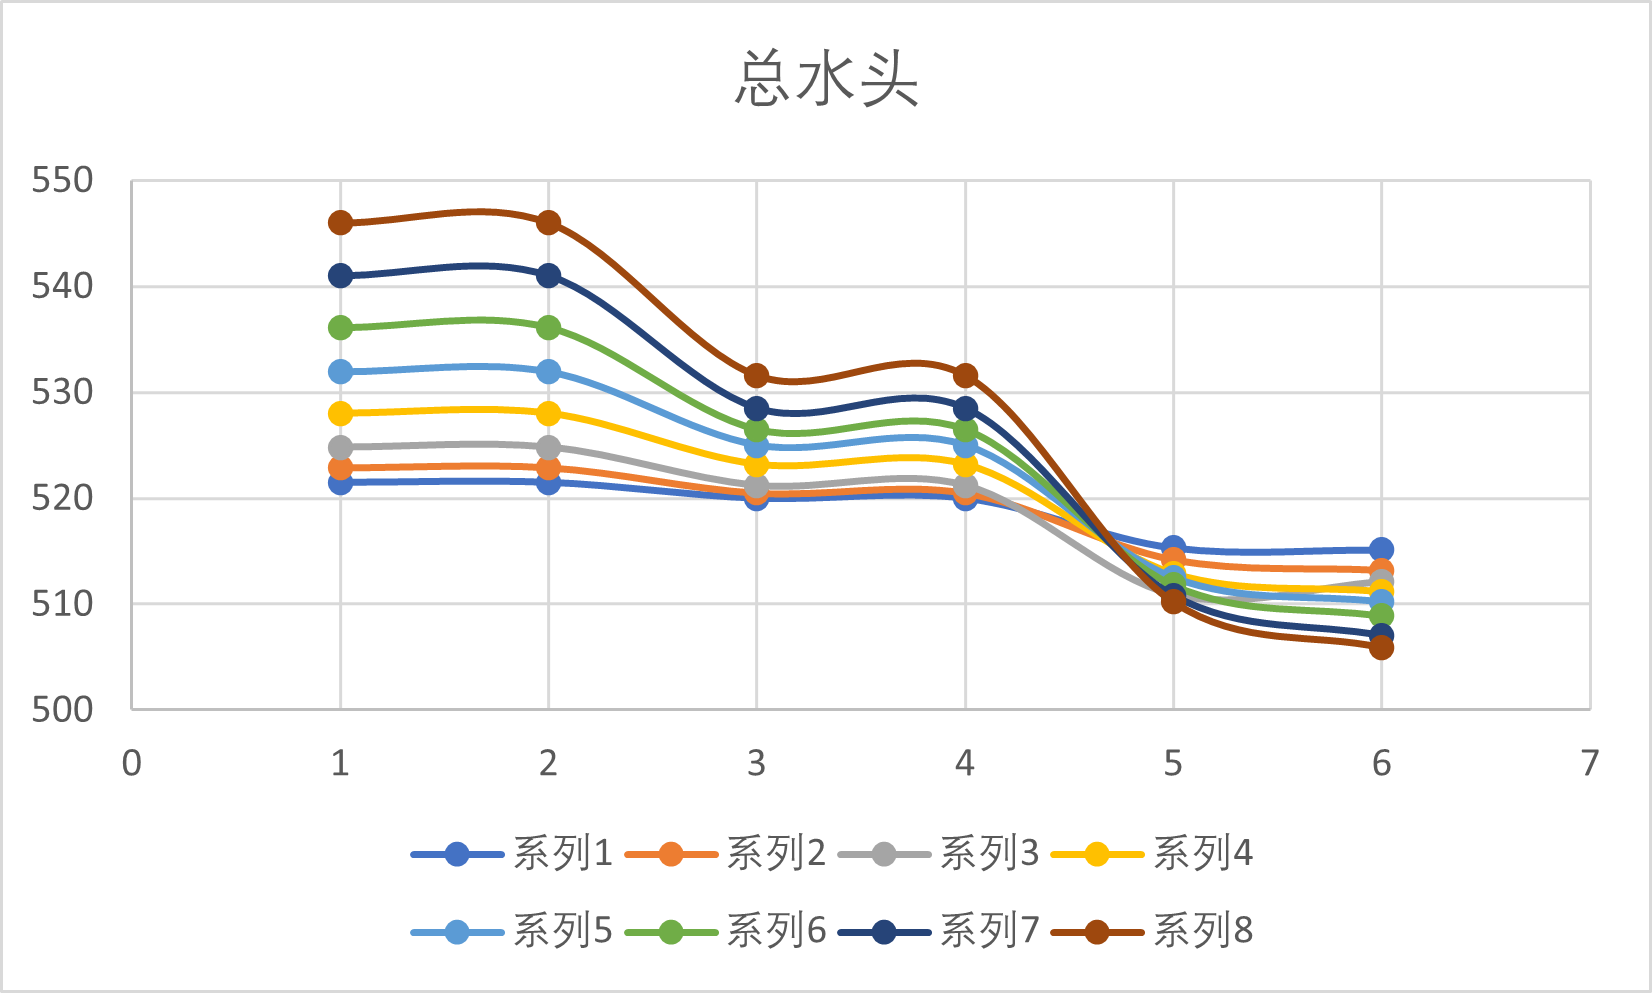
\includegraphics[width=0.95\textwidth]{2-1.png}
\end{figure}
\begin{figure}[!h]
	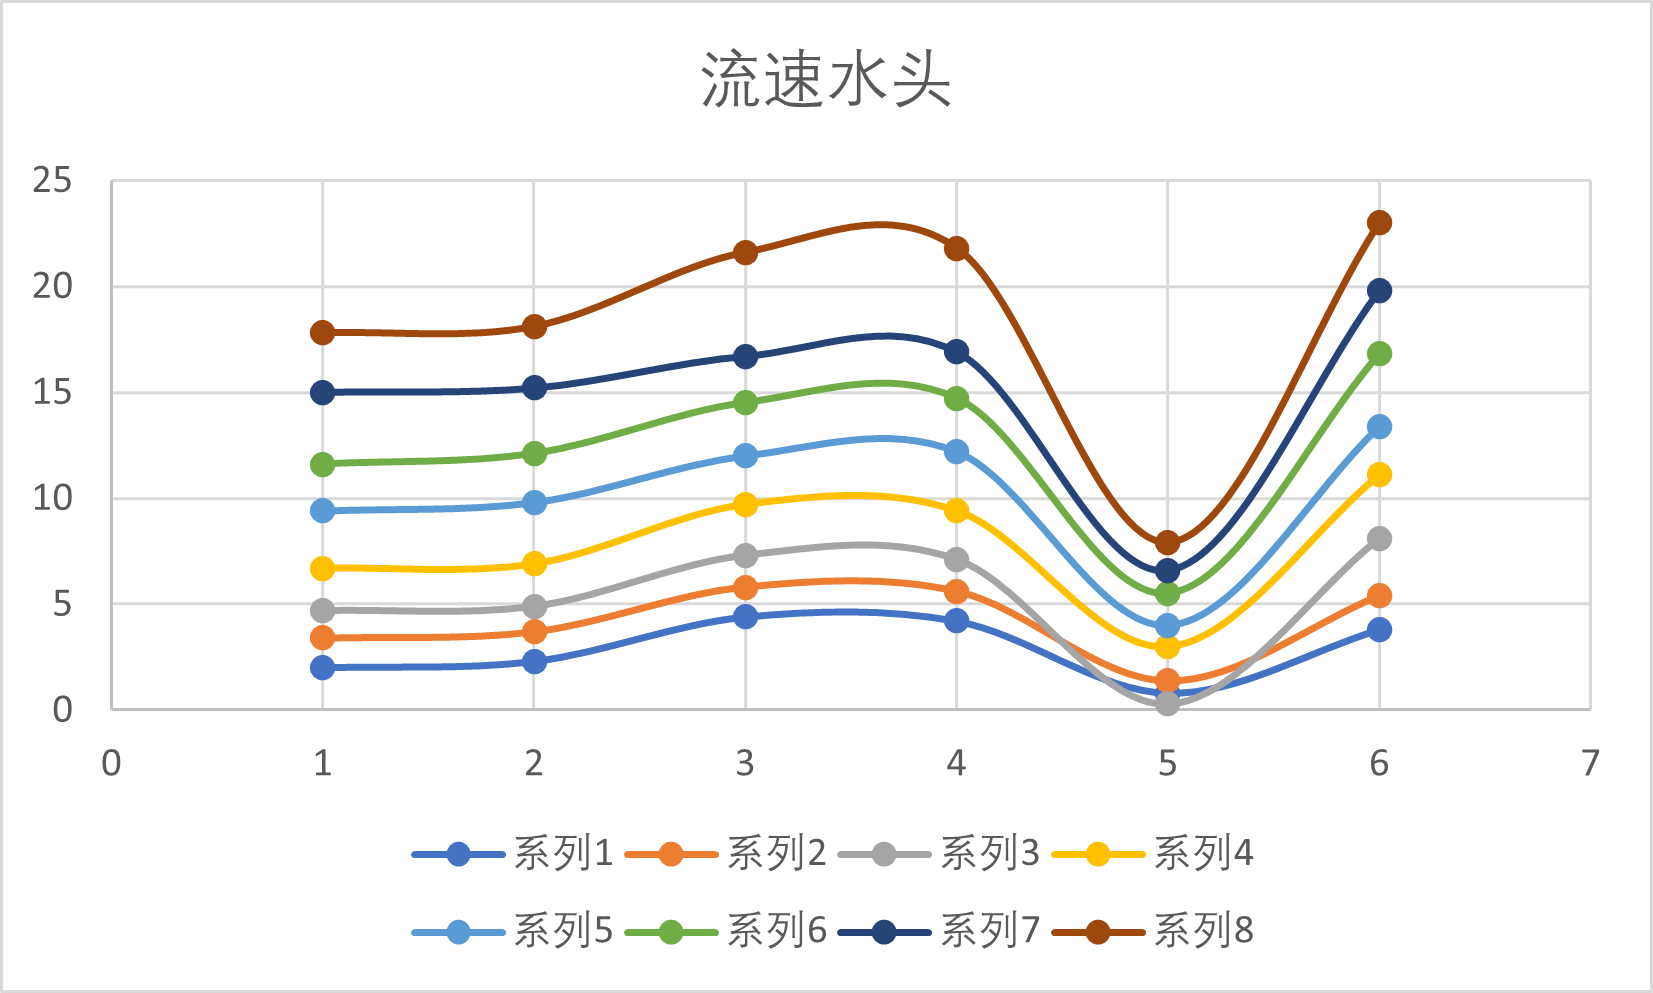
\includegraphics[width=0.95\textwidth]{2-2.png}
\end{figure}
\begin{figure}[!h]
	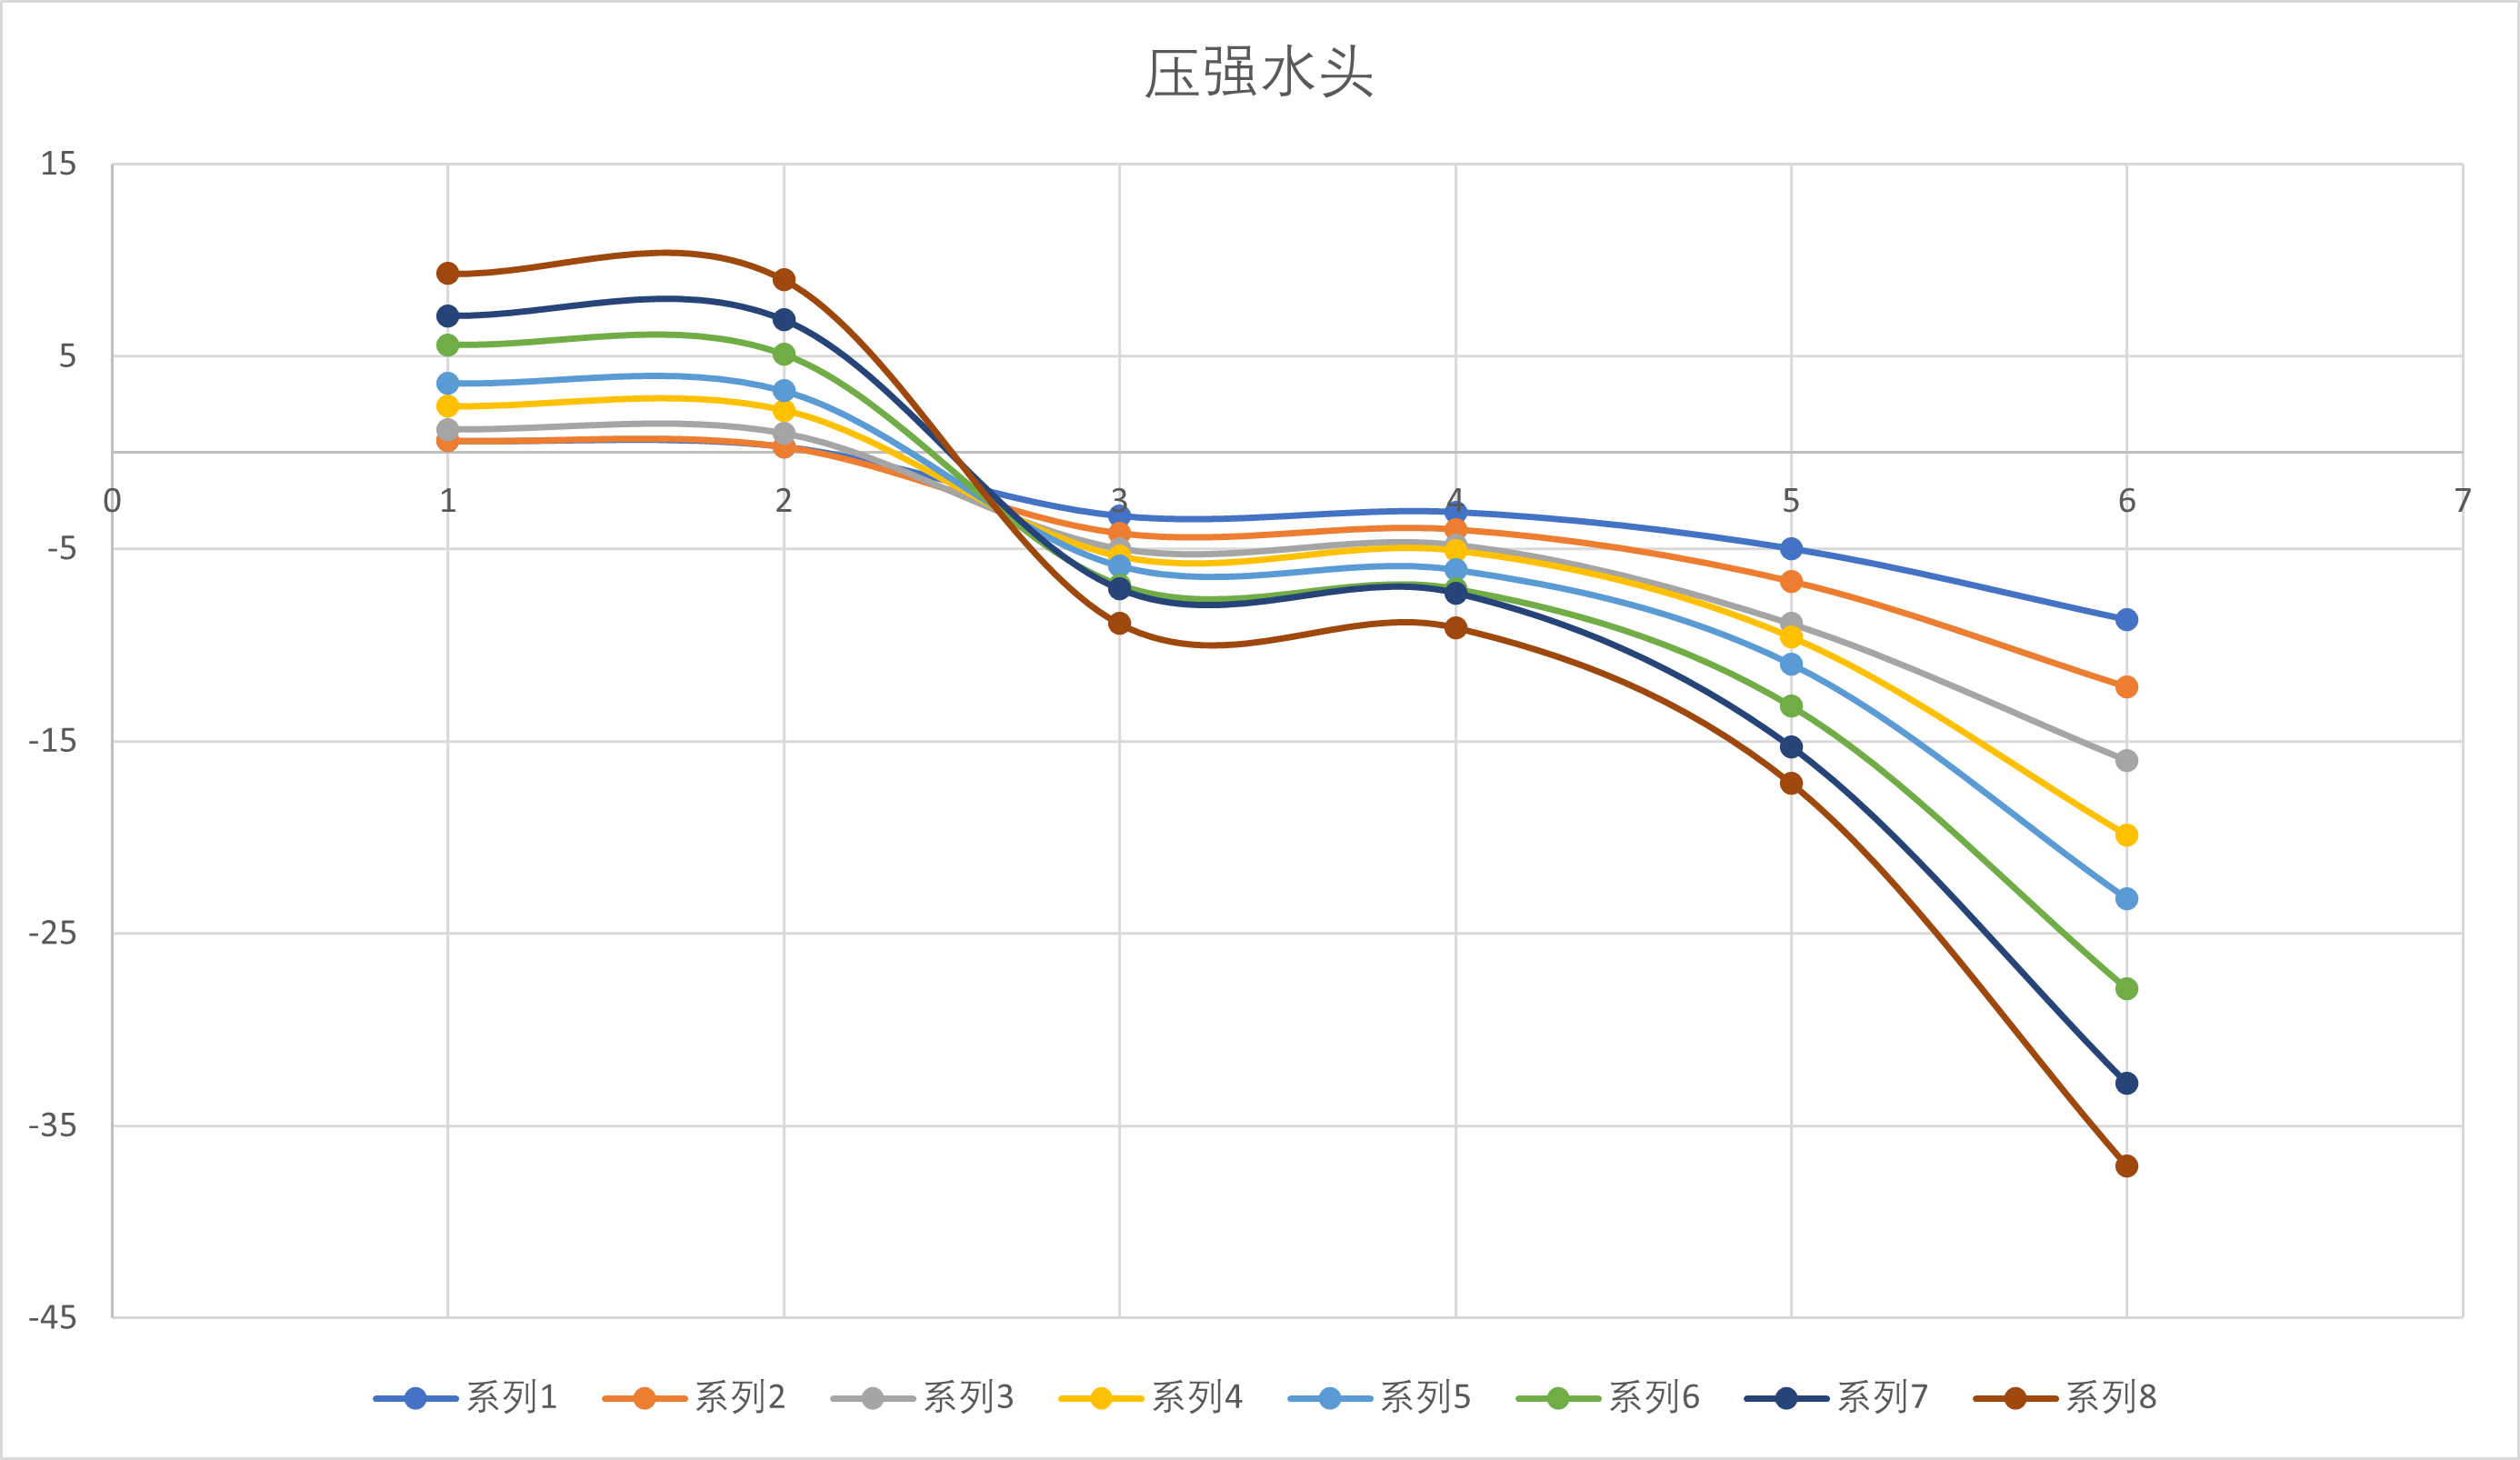
\includegraphics[width=0.95\textwidth]{2-3.png}
\end{figure}\par
\newpage
(3)运用伯努利方程进行分析,解释各水头的变化规律,例如:
\begin{enumerate}
	\item 可以看出能量损失沿着流体流动的方向是增大的;
	\item 11号处和13号处,其位置水头相同,但11号处比13号处的压强水头大,这是由于管径变细,流速增快,压强水头转变为流速水头;
	\item 实验结果还验证了连续方程,对于不可压缩流体的稳定流动,当流量一定时,管径粗的地方流速小,细的地方流速大;
	\item 沿程阻力损失与管径、流速和流动距离的关系(达西公式)。
\end{enumerate}
\begin{enumerate}
	\item 越靠近水泵的地方流速越大证明了管壁的摩擦。
	\item 总水头随着流动方向降低证明了能量损失。
	\item 随着流速增大能量损失速度加快,验证了达西公式。
\end{enumerate}
\par
2.测速实验\par
计算出毕托管各点的轴心速度和平均速度。(能量方程实验管上六组测压管的任一组都相当于一个毕托管,可测得管内的流体速度,由于本实验台将总水头测压管置于能量方程实验管的轴线,所以测得的动压头代表了轴心处的最大流速)
\begin{table}[!h]
	\renewcommand\arraystretch{1.7}
	\centering
	\begin{tabularx}{\textwidth}{|c|X|X|X|X|X|X|X|X|X|}
	\hline
	\multicolumn{2}{|c|}{截面序号/流量计流量/($\text{L}\cdot\text{min}^{-1}$)} & 0.5 & 0.65 & 0.8 & 0.95 & 1.1 & 1.25 & 1.4 & 1.55 \\ \hline
	\multirow{6}{*}{流速/(ms$^{-1}$)}&1 & 0.0392 & 0.06664 & 0.09212 & 0.13132 & 0.18424 & 0.22736 & 0.294 & 0.34888 \\ \cline{2-10}
	&2 & 0.04508 & 0.07252 & 0.09604 & 0.13524 & 0.19208 & 0.23716 & 0.29792 & 0.35476 \\ \cline{2-10}
	&3 & 0.08624 & 0.11368 & 0.14308 & 0.19012 & 0.2352 & 0.2842 & 0.32732 & 0.42336 \\ \cline{2-10}
	&4 & 0.08232 & 0.10976 & 0.13916 & 0.18424 & 0.23912 & 0.28812 & 0.33124 & 0.42728 \\ \cline{2-10}
	&5 & 0.01568 & 0.02744 & 0.00588 & 0.0588 & 0.0784 & 0.1078 & 0.12936 & 0.15484 \\ \cline{2-10}
	&6 & 0.07448 & 0.10584 & 0.15876 & 0.21756 & 0.26264 & 0.32928 & 0.38808 & 0.4508 \\ \hline
	\multicolumn{2}{|c|}{平均速度/(ms$^{-1}$)} &0.05717	&0.08265& 0.10584&0.15288&0.19861&0.24565&0.29465&0.35999\\
	\hline
	\end{tabularx}
\end{table}\par
\newpage
【实验思考题:选做感兴趣的题目或内容】\\
\begin{question}
	测压管水头线和总水头线的沿程变化趋势有何不同?为什么?
	\tcblower
	水流量较大时总水头下降较测压管水头下降更快。原因是管内壁有摩擦,使得能量有损耗
	故总水头下降较测压管水头下降更快。
\end{question}

\begin{question}
	流量增加,测压管水头线变化趋势如何变化?为什么?
	\tcblower
	水流量较大时测压管水头下降加快。原因是此时流管内部出现了湍流,使得流体产生了垂直于管壁的速度。
\end{question}

\begin{question}
	管中心流速与平均流速有何不同?为什么管中心流速总是大于管内平均流速?层流和湍流条件下,管中心流速和管内平均流速的差异如何变化?
	\tcblower
	管中心流速总是大于管内平均流速,原因是管中心距管壁最远,大于周围与管壁摩擦的水流的速度,故大于平均速度。湍流情况下
	管中心速度与平均速度的比值较层流情况下降。
\end{question}

\begin{question}
	毕托管测得流速与椭圆齿轮流量计得到值一致吗?为什么?
	\tcblower
	不一致,因为椭圆齿轮流量计对水流阻力远大于毕托管故流量计测得流速小于毕托管测得流速
\end{question}

\begin{question}
	摩擦压降是否与理论公式相符?
	\tcblower
	不相符,因为此时管内出现了湍流,使得超出了公式的适用范围。
\end{question}

\begin{question}
	实验数据能否判断管内是稳定流动还是湍流?
	\tcblower
	可以,只需要观察4号和5号测压管与6号和7号的液面是否相平,只要不相平便证明管内出现了湍流。
\end{question}

\begin{question}
	若回路没调水平,对实验结果有何影响?能否扣除?
	\tcblower
	会导致总水头测量失误,可以扣除,只需要记录流速为0时的液面高度,后续计算压力水头和流速水头的时候计算高度差即可。
\end{question}
\clearpage
% ---------------------------------------------------------------------
%   参考文献
%   注:使用参考文献时应按照xelatex->bibtex->xelatex->xelatex顺序进行编译
\phantomsection
%\addcontentsline{toc}{section}{参考文献}
\bibliographystyle{unsrt}
\bibliography{myref}
%\begin{thebibliography}{9}
	%\bibitem{ref1} 凤飞龙,黄育红,金蔚,王公正,崔致远,“外推法计算冰的熔解热的理论依据及Matlab实现方案”,《大学物理》,第42卷,第2期
%\end{thebibliography}


\clearpage
\appendix
\appendixpage
\addappheadtotoc
\subsection*{原件扫描}
\includepdf[pages=-]{实验2原件.pdf}
\subsection*{原始数据}
\includepdf[pages=-]{实验2数据.pdf}
\subsection*{桌面}
\begin{figure}[!h]
	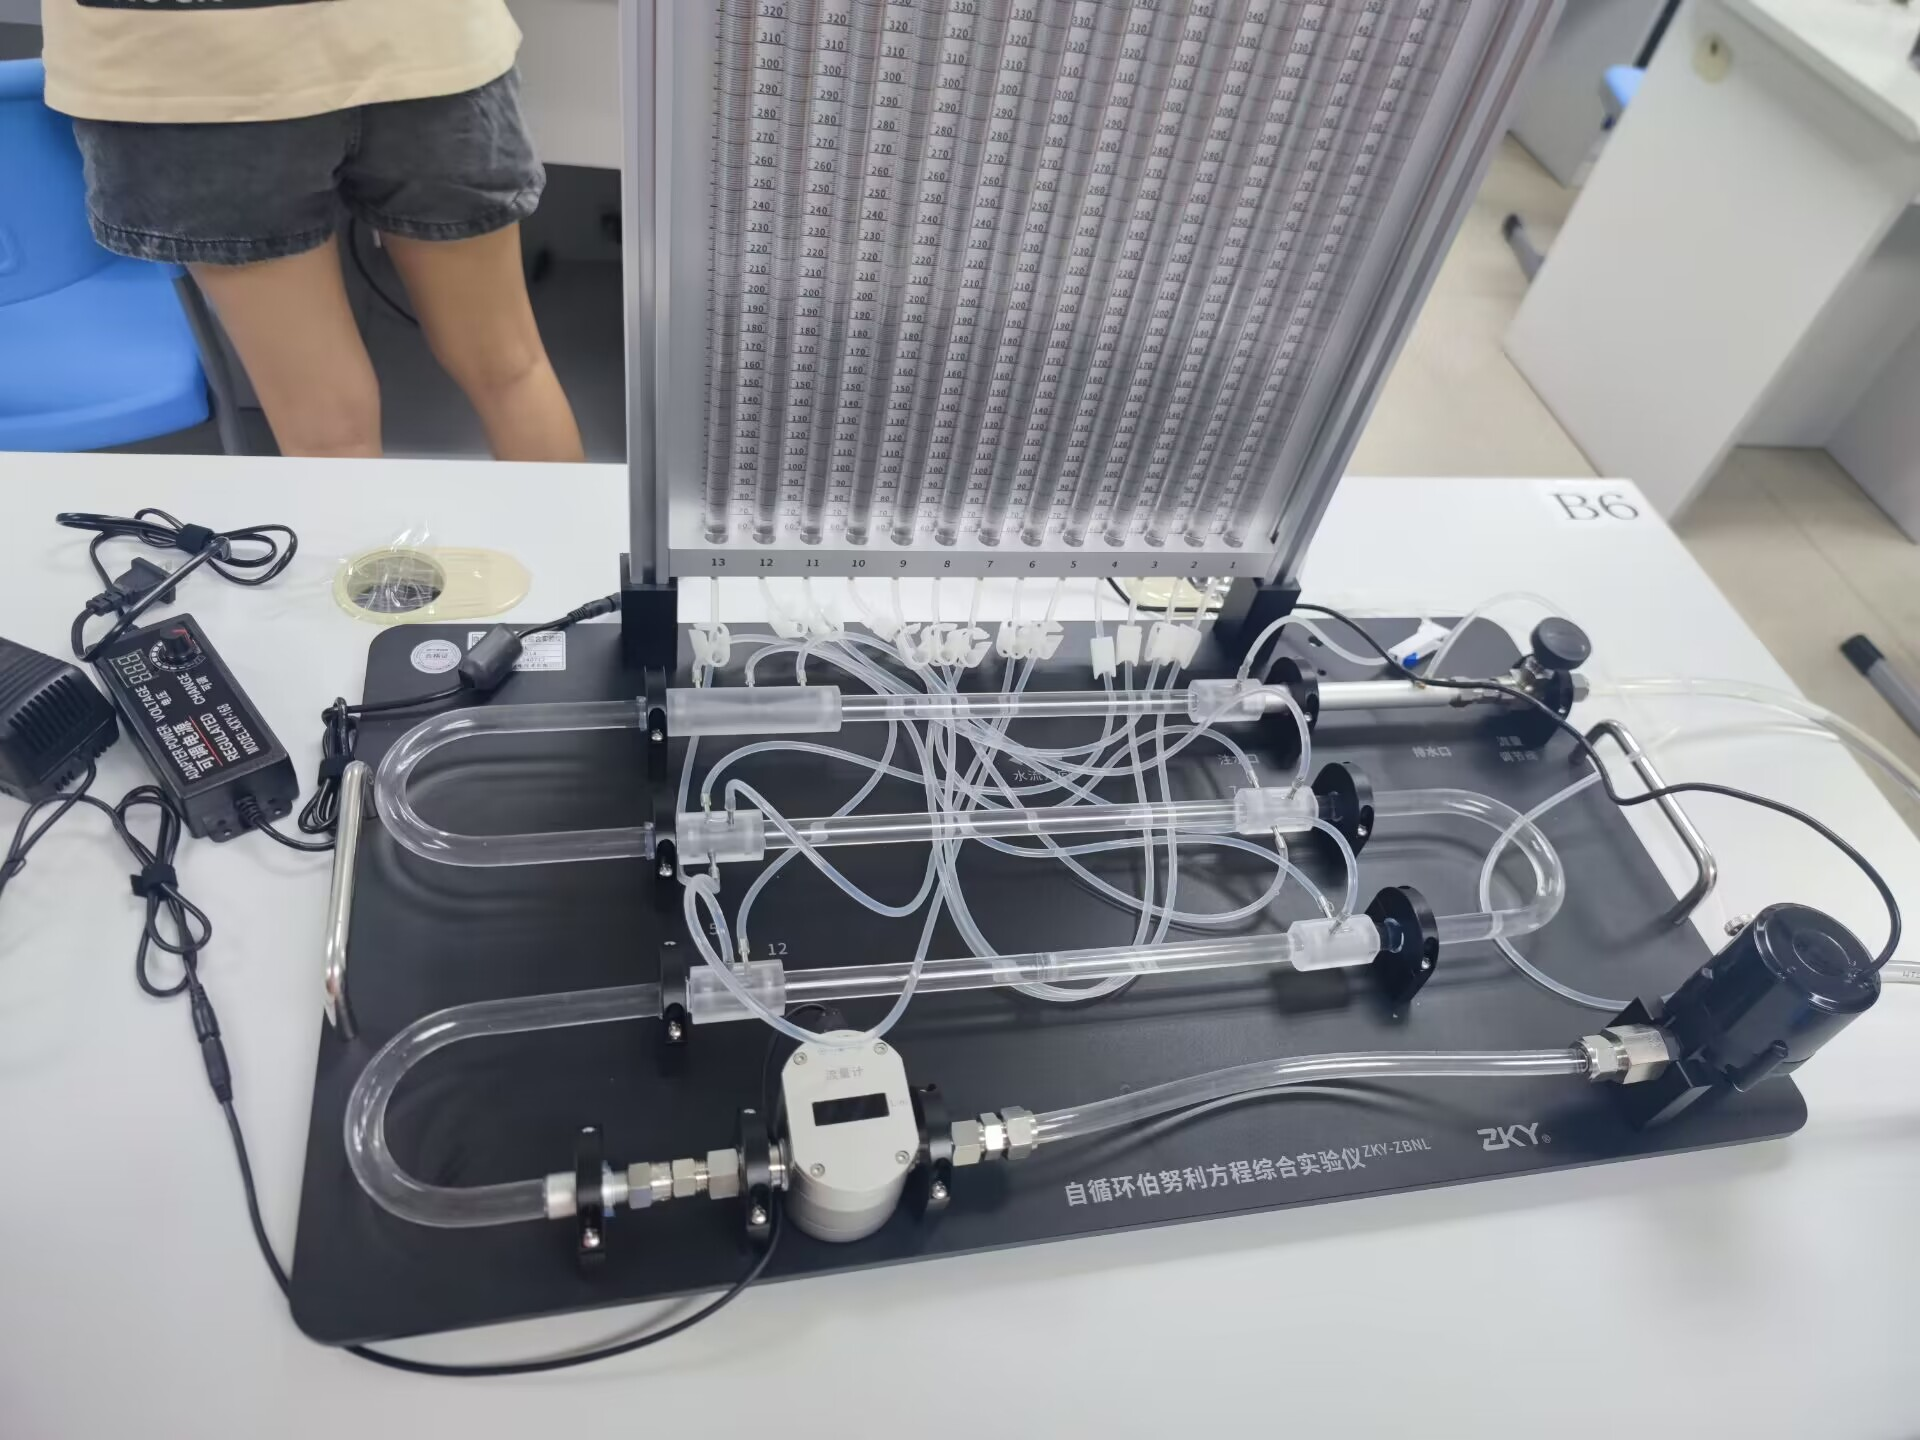
\includegraphics[width=0.95\textwidth]{实验2桌面.jpg}
\end{figure}
\end{document}

